\documentclass[a4paper,12pt]{article}
\usepackage{czech}
\usepackage[utf8]{inputenc}
\usepackage{a4wide}
\usepackage[dvipdfm]{graphicx}
\usepackage{graphics}
\usepackage{indentfirst}
\usepackage{fancyhdr}
\usepackage{setspace}
\usepackage{amsmath}
\usepackage{amssymb}
\usepackage{epsfig}

%%\usepackage{nopageno}
%%\usepackage{txfonts}
\usepackage[usenames]{color}
\begin{document}



\section{Úkol}
\begin{enumerate}
\item S použitím spektra rtuti zkalibrujte hranolový spektrometr. Pro vyloučení hrubých chyb vyneste kalibrační křivku ikhend do grafu.
\item Ověřte vlnové délky sodíkových dubletů (alespoň tří)
\item Na základě pozorování sodíkových dubletů diskutujte rozlišovací schopnost spektrometru. Diskutujte přesnost takto určené rozlišovací schopnosti.
\item Prohlédněte sis pektra výbojek čar $H_\alpha$, $H_\beta$, $H_\gamma$ Balmerovy serie vodíkového spektra. Vypočítejte Rydbergovu konstantu.
\end{enumerate}

\section{Teorie}
Spektrometr je zařízení pro určení vlnové délky světla. Běžně se používá mřížkový nebo hranolový. Přístroj využívá různého lomu (odrazu) na hranolu (mřížce) pro různé vlnové délky světla.

Vlnové délky spektrálních čar vodíku se řídí dle \cite{text} vztahem
\begin{eqnarray}
\lambda = \frac{n^2}{R\left(\left(\frac{n}{2}\right)^2-1\right) },
\label{Ry}
\end{eqnarray}
kde R je Rydbergova konstanta ($1.0973 \cdot 10^7 \mbox{m}^{-1} $) a $n$ je přirozené číslo. Ve viditelném sektru můžeme pozorovat spektrální čáry pro n=3,4,5,6.

\section{Měření}
\subsection{Kalibrace}
Nejprve jsem za pomoci rtuťové výbojky provedl kalibraci spektrometru. Odečtené hodnoty ze stupnice jsem poronal se známými hodnotami vlnových délek těchto čar. Výslednou závislost jsem proložil polynemom pátého stupně, který má předpis
\begin{eqnarray}
\lambda(x)=((((3.90\cdot 10^{-15}x-2.46\cdot 10^{-11})x+ 6.73\cdot 10^{-8})x-7.49\cdot 10^{-5})x+0.0840)x+366
\label{P}
\end{eqnarray}.
Tento polynom je použit pro výpočet vlnových délek spektrálních čar ve zbytku protokolu.
Naměřené hodnoty jsou shrnuty s hodnotami tabelovými a dopočtenými za pomoci polynomu \ref{P} v tabulce \ref{THg}. Vynesená závislost je na obrázku (\ref{GHg}).

\begin{table}
$$
\begin{array}{|c|c|c|}
\hline
\lambda_t/\mbox{nm}&    x&  \lambda/\mbox{nm} \\ \hline
404.7&  678&    404.6 \\ \hline
407.8&  744&    407.9 \\ \hline
433.9&  1200&   433.8 \\ \hline
434.8&  1216&   434.8 \\ \hline
491.6&  1890&   491.7 \\ \hline
546.1&  2308&   545.8 \\ \hline
577.0&  2488&   577.2 \\ \hline
579.1&  2500&   579.5 \\ \hline
607.3&  2630&   607.1 \\ \hline
612.3&  2652&   612.2 \\ \hline
623.4&  2698&   623.4 \\ \hline
671.6&  2870&   671.7 \\ \hline
690.7&  2928&   690.7 \\ \hline
\end{array}
$$
\caption{Naměřené honodty pro Hg výbojku.}
\label{THg}
\end{table}

\begin{figure}[h!]
% GNUPLOT: LaTeX picture with Postscript
\begingroup
  \makeatletter
  \providecommand\color[2][]{%
    \GenericError{(gnuplot) \space\space\space\@spaces}{%
      Package color not loaded in conjunction with
      terminal option `colourtext'%
    }{See the gnuplot documentation for explanation.%
    }{Either use 'blacktext' in gnuplot or load the package
      color.sty in LaTeX.}%
    \renewcommand\color[2][]{}%
  }%
  \providecommand\includegraphics[2][]{%
    \GenericError{(gnuplot) \space\space\space\@spaces}{%
      Package graphicx or graphics not loaded%
    }{See the gnuplot documentation for explanation.%
    }{The gnuplot epslatex terminal needs graphicx.sty or graphics.sty.}%
    \renewcommand\includegraphics[2][]{}%
  }%
  \providecommand\rotatebox[2]{#2}%
  \@ifundefined{ifGPcolor}{%
    \newif\ifGPcolor
    \GPcolorfalse
  }{}%
  \@ifundefined{ifGPblacktext}{%
    \newif\ifGPblacktext
    \GPblacktexttrue
  }{}%
  % define a \g@addto@macro without @ in the name:
  \let\gplgaddtomacro\g@addto@macro
  % define empty templates for all commands taking text:
  \gdef\gplbacktext{}%
  \gdef\gplfronttext{}%
  \makeatother
  \ifGPblacktext
    % no textcolor at all
    \def\colorrgb#1{}%
    \def\colorgray#1{}%
  \else
    % gray or color?
    \ifGPcolor
      \def\colorrgb#1{\color[rgb]{#1}}%
      \def\colorgray#1{\color[gray]{#1}}%
      \expandafter\def\csname LTw\endcsname{\color{white}}%
      \expandafter\def\csname LTb\endcsname{\color{black}}%
      \expandafter\def\csname LTa\endcsname{\color{black}}%
      \expandafter\def\csname LT0\endcsname{\color[rgb]{1,0,0}}%
      \expandafter\def\csname LT1\endcsname{\color[rgb]{0,1,0}}%
      \expandafter\def\csname LT2\endcsname{\color[rgb]{0,0,1}}%
      \expandafter\def\csname LT3\endcsname{\color[rgb]{1,0,1}}%
      \expandafter\def\csname LT4\endcsname{\color[rgb]{0,1,1}}%
      \expandafter\def\csname LT5\endcsname{\color[rgb]{1,1,0}}%
      \expandafter\def\csname LT6\endcsname{\color[rgb]{0,0,0}}%
      \expandafter\def\csname LT7\endcsname{\color[rgb]{1,0.3,0}}%
      \expandafter\def\csname LT8\endcsname{\color[rgb]{0.5,0.5,0.5}}%
    \else
      % gray
      \def\colorrgb#1{\color{black}}%
      \def\colorgray#1{\color[gray]{#1}}%
      \expandafter\def\csname LTw\endcsname{\color{white}}%
      \expandafter\def\csname LTb\endcsname{\color{black}}%
      \expandafter\def\csname LTa\endcsname{\color{black}}%
      \expandafter\def\csname LT0\endcsname{\color{black}}%
      \expandafter\def\csname LT1\endcsname{\color{black}}%
      \expandafter\def\csname LT2\endcsname{\color{black}}%
      \expandafter\def\csname LT3\endcsname{\color{black}}%
      \expandafter\def\csname LT4\endcsname{\color{black}}%
      \expandafter\def\csname LT5\endcsname{\color{black}}%
      \expandafter\def\csname LT6\endcsname{\color{black}}%
      \expandafter\def\csname LT7\endcsname{\color{black}}%
      \expandafter\def\csname LT8\endcsname{\color{black}}%
    \fi
  \fi
  \setlength{\unitlength}{0.0500bp}%
  \begin{picture}(7200.00,5040.00)%
    \gplgaddtomacro\gplbacktext{%
      \csname LTb\endcsname%
      \put(1078,704){\makebox(0,0)[r]{\strut{} 400}}%
      \put(1078,1383){\makebox(0,0)[r]{\strut{} 450}}%
      \put(1078,2061){\makebox(0,0)[r]{\strut{} 500}}%
      \put(1078,2740){\makebox(0,0)[r]{\strut{} 550}}%
      \put(1078,3418){\makebox(0,0)[r]{\strut{} 600}}%
      \put(1078,4097){\makebox(0,0)[r]{\strut{} 650}}%
      \put(1078,4775){\makebox(0,0)[r]{\strut{} 700}}%
      \put(1210,484){\makebox(0,0){\strut{} 500}}%
      \put(2342,484){\makebox(0,0){\strut{} 1000}}%
      \put(3474,484){\makebox(0,0){\strut{} 1500}}%
      \put(4605,484){\makebox(0,0){\strut{} 2000}}%
      \put(5737,484){\makebox(0,0){\strut{} 2500}}%
      \put(6869,484){\makebox(0,0){\strut{} 3000}}%
      \put(308,2739){\rotatebox{-270}{\makebox(0,0){\strut{}$\lambda$/nm}}}%
      \put(4039,154){\makebox(0,0){\strut{}x}}%
    }%
    \gplgaddtomacro\gplfronttext{%
    }%
    \gplbacktext
    \put(0,0){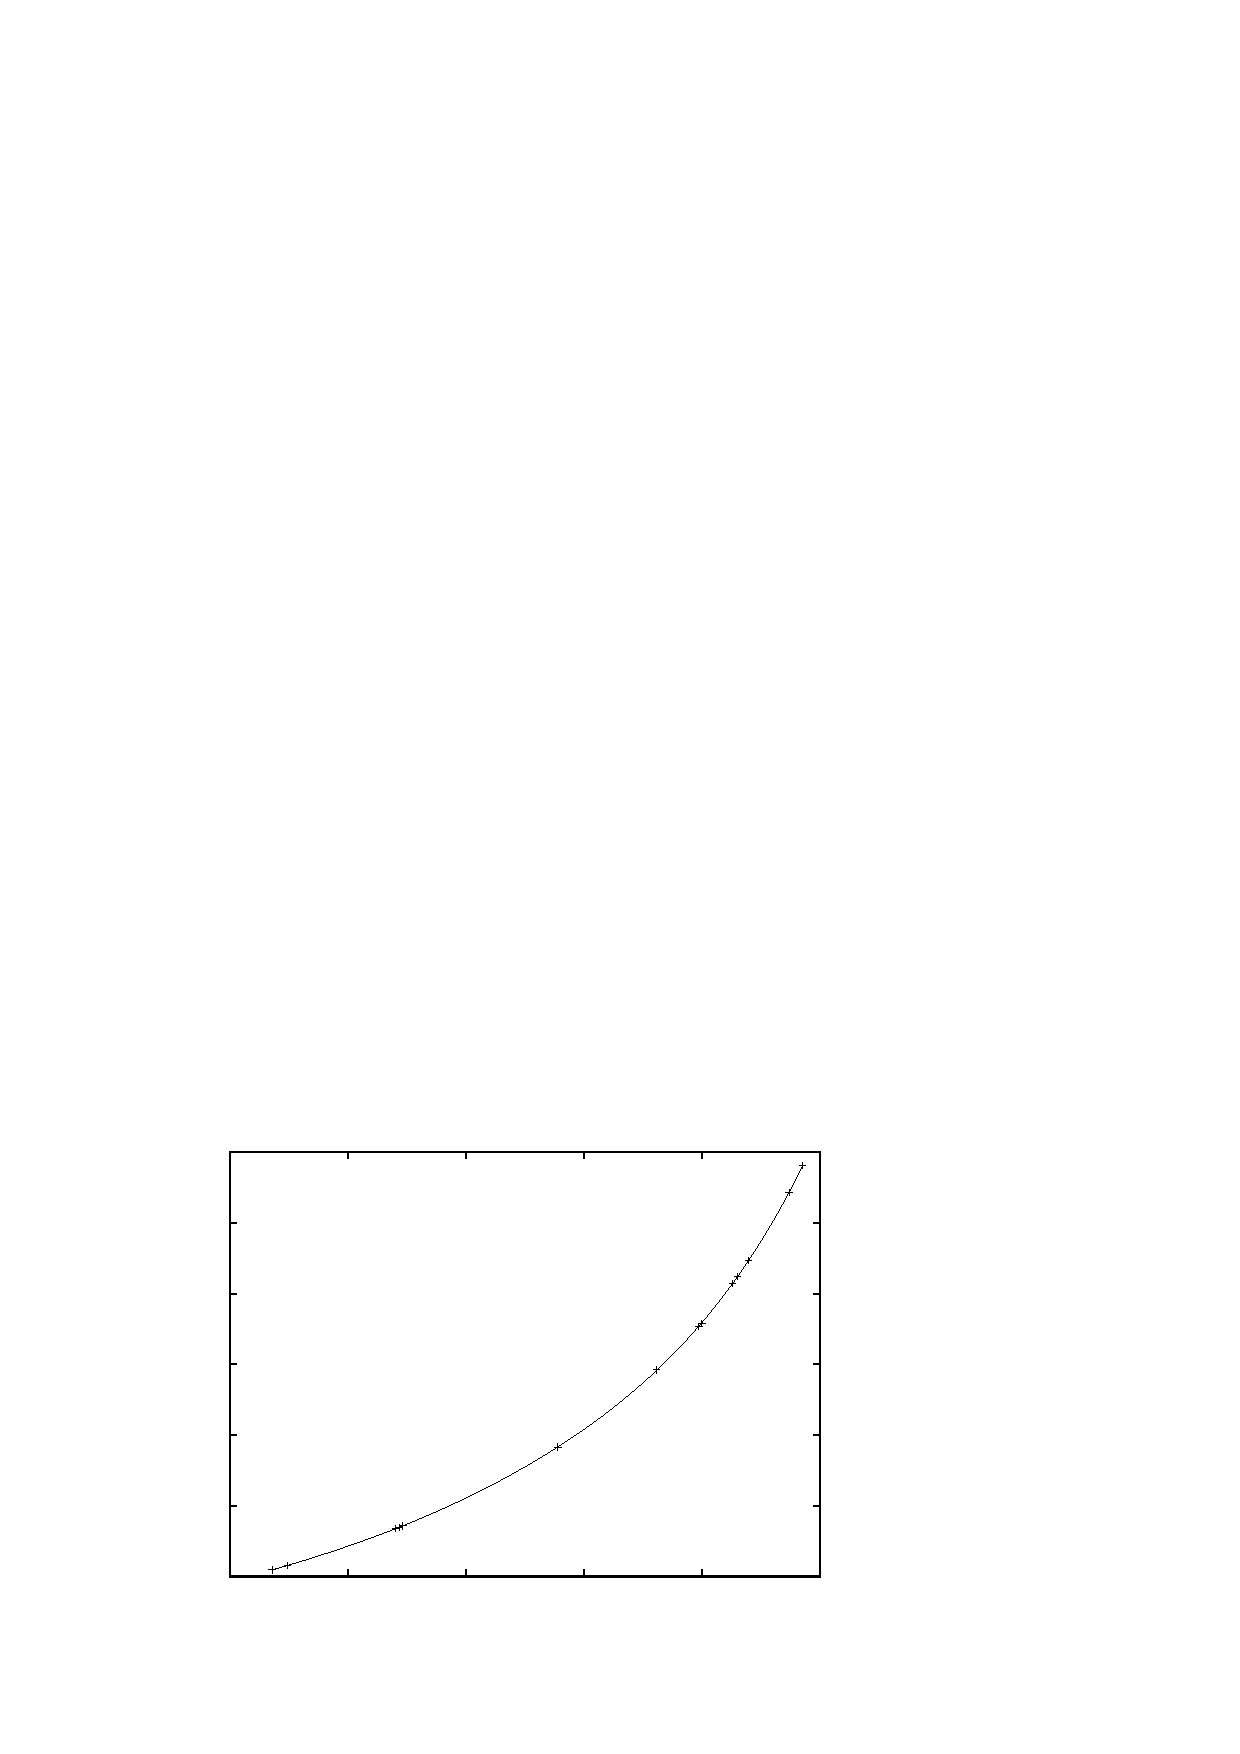
\includegraphics{GHg}}%
    \gplfronttext
  \end{picture}%
\endgroup

\caption{Kalibrační křivka spektrometru.}
\label{GHg}
\end{figure}

\subsection{Na}
Proměřil jsem tři sodíkové dublety. Naměřené hodnoty jsou spolu s tabelovýmo shrnuty v tabulce ref{TNa}. Jak je vidět na hodnotách, poloha dubletu se od tabelových hodnot liší až v řádu setim desetin nanemetru. Všechny dublety byly dobře rozpoznatelné, takže rozlišovací schopnost spektrometru se pohybuje v okolí rozdílu nejbližších čar, který je 0.04 nm. Měřitelnost jejich rozdílu je však minimálně o řád nižší.

\begin{table}
$$
\begin{array}{|c|c|c|}
\hline
x&  \lambda/\mbox{nm}&  \lambda_t/\mbox{nm} \\ \hline
2550&   589.6&  589.592 \\ \hline
2548&   589.2&  588.995 \\ \hline
2669&   616.3&  616.076 \\ \hline
2667&   615.8&  615.423 \\ \hline
2443&   568.7&  568.861 \\ \hline
2438&   567.8&  568.822 \\ \hline
\end{array}
$$
\caption{Hodnoty sodíkových dupletů}
\label{TNa}
\end{table}


\subsection{Další plyny}
Dále jsem ptoměřil 5 dalších plynů. Naměřené hodnoty jsou v tabulkách \ref{THe}, \ref{TNe}, \ref{TAr}, \ref{TCO2}. U vzácných plynů jsou pro srovnání uvedeny i tabelové hodnoty. U sloučenin se již projevil vliv vazeb na spektrum a tak vzniklo částečně spojité spektrum s jasnými hranami, jejiž hodnoty jsou uvedeny v tabulkách.

\begin{table}
$$
\begin{array}{|c|c|c|}
\hline
x&  \lambda/\mbox{nm}&  \lambda_t/\mbox{nm} \\ \hline
2539&   587.3&  587.562 \\ \hline
2860&   668.6&  667.815 \\ \hline
2972&   706.1&  706.519 \\ \hline
2290&   543.0&  541.115 \\ \hline
2008&   505.0&  504.774 \\ \hline
1978&   708.2&  501.568 \\ \hline
1892&   492.0&  492.193 \\ \hline
1680&   471.0&  471.315 \\ \hline
1390&   447.0&  447.168 \\ \hline
\end{array}
$$
\caption{Spektrální čáry He výbojky}
\label{THe}
\end{table}


\begin{table}
$$
\begin{array}{|c|c|c|}
\hline
x&  \lambda/\mbox{nm}&  \lambda_t/\mbox{nm} \\ \hline
1678&   470.8&  470.883 \\ \hline
1994&   503.3&  503.133 \\ \hline
2220&   532.5&  533.078 \\ \hline
2229&   533.8&  534.109 \\ \hline
2266&   539.3&  540.036 \\ \hline
2483&   576.2&  576.442 \\ \hline
2528&   585.1&  583.249 \\ \hline
2572&   594.2&  594.483 \\ \hline
2642&   609.9&  609.616 \\ \hline
2660&   614.1&  614.306 \\ \hline
2712&   626.9&  626.649 \\ \hline
2762&   640.1&  640.223 \\ \hline
2860&   668.6&  667.828 \\ \hline
\end{array}
$$
\caption{Spektrální čáry Ne výbojky}
\label{TNe}
\end{table}

\begin{table}
$$
\begin{array}{|c|c|c|}
\hline
x&  \lambda/\mbox{nm}&  \lambda_t/\mbox{nm} \\ \hline
968&    419.7&  419.832 \\ \hline
1193&   433.3&  433.356 \\ \hline
1435&   450.5&  451.073 \\ \hline
1662&   469.3&  470.232 \\ \hline
2114&   518.0&  518.774 \\ \hline
2328&   549.0&  549.587 \\ \hline
2396&   560.3&  560.673 \\ \hline
2556&   590.8&  591.208 \\ \hline
2612&   603.0&  603.212 \\ \hline
2768&   614.7&  614.544 \\ \hline
2945&   696.4&  696.543 \\ \hline
\end{array}
$$
\caption{Spektrální čáry Ar výbojky}
\label{TAr}
\end{table}

\begin{table}
$$
\begin{array}{|c|c|}
\hline
x&  \lambda/\mbox{nm} \\ \hline
1436&   450.5 \\ \hline
1810&   483.4 \\ \hline
2126&   519.6 \\ \hline
2398&   560.7 \\ \hline
2631&   607.3 \\ \hline
2839&   662.2 \\ \hline
\end{array}
$$
\caption{Spektrální čáry CO2 výbojky}
\label{TCO2}
\end{table}


\subsection{H}
Nakonec jsem proměřil čárové spektrum vodíku. Dobře viditelné byli pouze dvě čáry. Třetí ve fialové části spektra byla pouze znatelná a určení její polohy je spíše intuitivní. Naměřené hodnoty jsem vynesl do grafu a proložil je křivkou odpovídající vztahu \ref{Ry}. Z fitu jsem odečet výslednou hodnotu Rydbergovy konstanty
\begin{eqnarray}
Ry=1.0973 \cdot 10^{-7}   \mbox{m}^{-1}
\end{eqnarray}
Závislost s proloženou křivkou je na obrázku \ref{GH}

\begin{table}
$$
\begin{array}{|c|c|c|}
\hline
x&  \lambda/\mbox{nm}&  \lambda_t/\mbox{nm} \\ \hline
2820&   656.5&  656.285 \\ \hline
1834&   485.8&  486.133 \\ \hline
1199&   433.7&  434.047 \\ \hline
\end{array}
$$
\caption{Spektrální čáry vodíku}
\label{TH}
\end{table}


\begin{figure}[h!]
% GNUPLOT: LaTeX picture with Postscript
\begingroup
  \makeatletter
  \providecommand\color[2][]{%
    \GenericError{(gnuplot) \space\space\space\@spaces}{%
      Package color not loaded in conjunction with
      terminal option `colourtext'%
    }{See the gnuplot documentation for explanation.%
    }{Either use 'blacktext' in gnuplot or load the package
      color.sty in LaTeX.}%
    \renewcommand\color[2][]{}%
  }%
  \providecommand\includegraphics[2][]{%
    \GenericError{(gnuplot) \space\space\space\@spaces}{%
      Package graphicx or graphics not loaded%
    }{See the gnuplot documentation for explanation.%
    }{The gnuplot epslatex terminal needs graphicx.sty or graphics.sty.}%
    \renewcommand\includegraphics[2][]{}%
  }%
  \providecommand\rotatebox[2]{#2}%
  \@ifundefined{ifGPcolor}{%
    \newif\ifGPcolor
    \GPcolorfalse
  }{}%
  \@ifundefined{ifGPblacktext}{%
    \newif\ifGPblacktext
    \GPblacktexttrue
  }{}%
  % define a \g@addto@macro without @ in the name:
  \let\gplgaddtomacro\g@addto@macro
  % define empty templates for all commands taking text:
  \gdef\gplbacktext{}%
  \gdef\gplfronttext{}%
  \makeatother
  \ifGPblacktext
    % no textcolor at all
    \def\colorrgb#1{}%
    \def\colorgray#1{}%
  \else
    % gray or color?
    \ifGPcolor
      \def\colorrgb#1{\color[rgb]{#1}}%
      \def\colorgray#1{\color[gray]{#1}}%
      \expandafter\def\csname LTw\endcsname{\color{white}}%
      \expandafter\def\csname LTb\endcsname{\color{black}}%
      \expandafter\def\csname LTa\endcsname{\color{black}}%
      \expandafter\def\csname LT0\endcsname{\color[rgb]{1,0,0}}%
      \expandafter\def\csname LT1\endcsname{\color[rgb]{0,1,0}}%
      \expandafter\def\csname LT2\endcsname{\color[rgb]{0,0,1}}%
      \expandafter\def\csname LT3\endcsname{\color[rgb]{1,0,1}}%
      \expandafter\def\csname LT4\endcsname{\color[rgb]{0,1,1}}%
      \expandafter\def\csname LT5\endcsname{\color[rgb]{1,1,0}}%
      \expandafter\def\csname LT6\endcsname{\color[rgb]{0,0,0}}%
      \expandafter\def\csname LT7\endcsname{\color[rgb]{1,0.3,0}}%
      \expandafter\def\csname LT8\endcsname{\color[rgb]{0.5,0.5,0.5}}%
    \else
      % gray
      \def\colorrgb#1{\color{black}}%
      \def\colorgray#1{\color[gray]{#1}}%
      \expandafter\def\csname LTw\endcsname{\color{white}}%
      \expandafter\def\csname LTb\endcsname{\color{black}}%
      \expandafter\def\csname LTa\endcsname{\color{black}}%
      \expandafter\def\csname LT0\endcsname{\color{black}}%
      \expandafter\def\csname LT1\endcsname{\color{black}}%
      \expandafter\def\csname LT2\endcsname{\color{black}}%
      \expandafter\def\csname LT3\endcsname{\color{black}}%
      \expandafter\def\csname LT4\endcsname{\color{black}}%
      \expandafter\def\csname LT5\endcsname{\color{black}}%
      \expandafter\def\csname LT6\endcsname{\color{black}}%
      \expandafter\def\csname LT7\endcsname{\color{black}}%
      \expandafter\def\csname LT8\endcsname{\color{black}}%
    \fi
  \fi
  \setlength{\unitlength}{0.0500bp}%
  \begin{picture}(7200.00,5040.00)%
    \gplgaddtomacro\gplbacktext{%
      \csname LTb\endcsname%
      \put(1078,704){\makebox(0,0)[r]{\strut{} 400}}%
      \put(1078,1383){\makebox(0,0)[r]{\strut{} 450}}%
      \put(1078,2061){\makebox(0,0)[r]{\strut{} 500}}%
      \put(1078,2740){\makebox(0,0)[r]{\strut{} 550}}%
      \put(1078,3418){\makebox(0,0)[r]{\strut{} 600}}%
      \put(1078,4097){\makebox(0,0)[r]{\strut{} 650}}%
      \put(1078,4775){\makebox(0,0)[r]{\strut{} 700}}%
      \put(1467,484){\makebox(0,0){\strut{} 3}}%
      \put(2753,484){\makebox(0,0){\strut{} 3.5}}%
      \put(4040,484){\makebox(0,0){\strut{} 4}}%
      \put(5326,484){\makebox(0,0){\strut{} 4.5}}%
      \put(6612,484){\makebox(0,0){\strut{} 5}}%
      \put(308,2739){\rotatebox{-270}{\makebox(0,0){\strut{}$\lambda$/nm}}}%
      \put(4039,154){\makebox(0,0){\strut{}n}}%
    }%
    \gplgaddtomacro\gplfronttext{%
    }%
    \gplbacktext
    \put(0,0){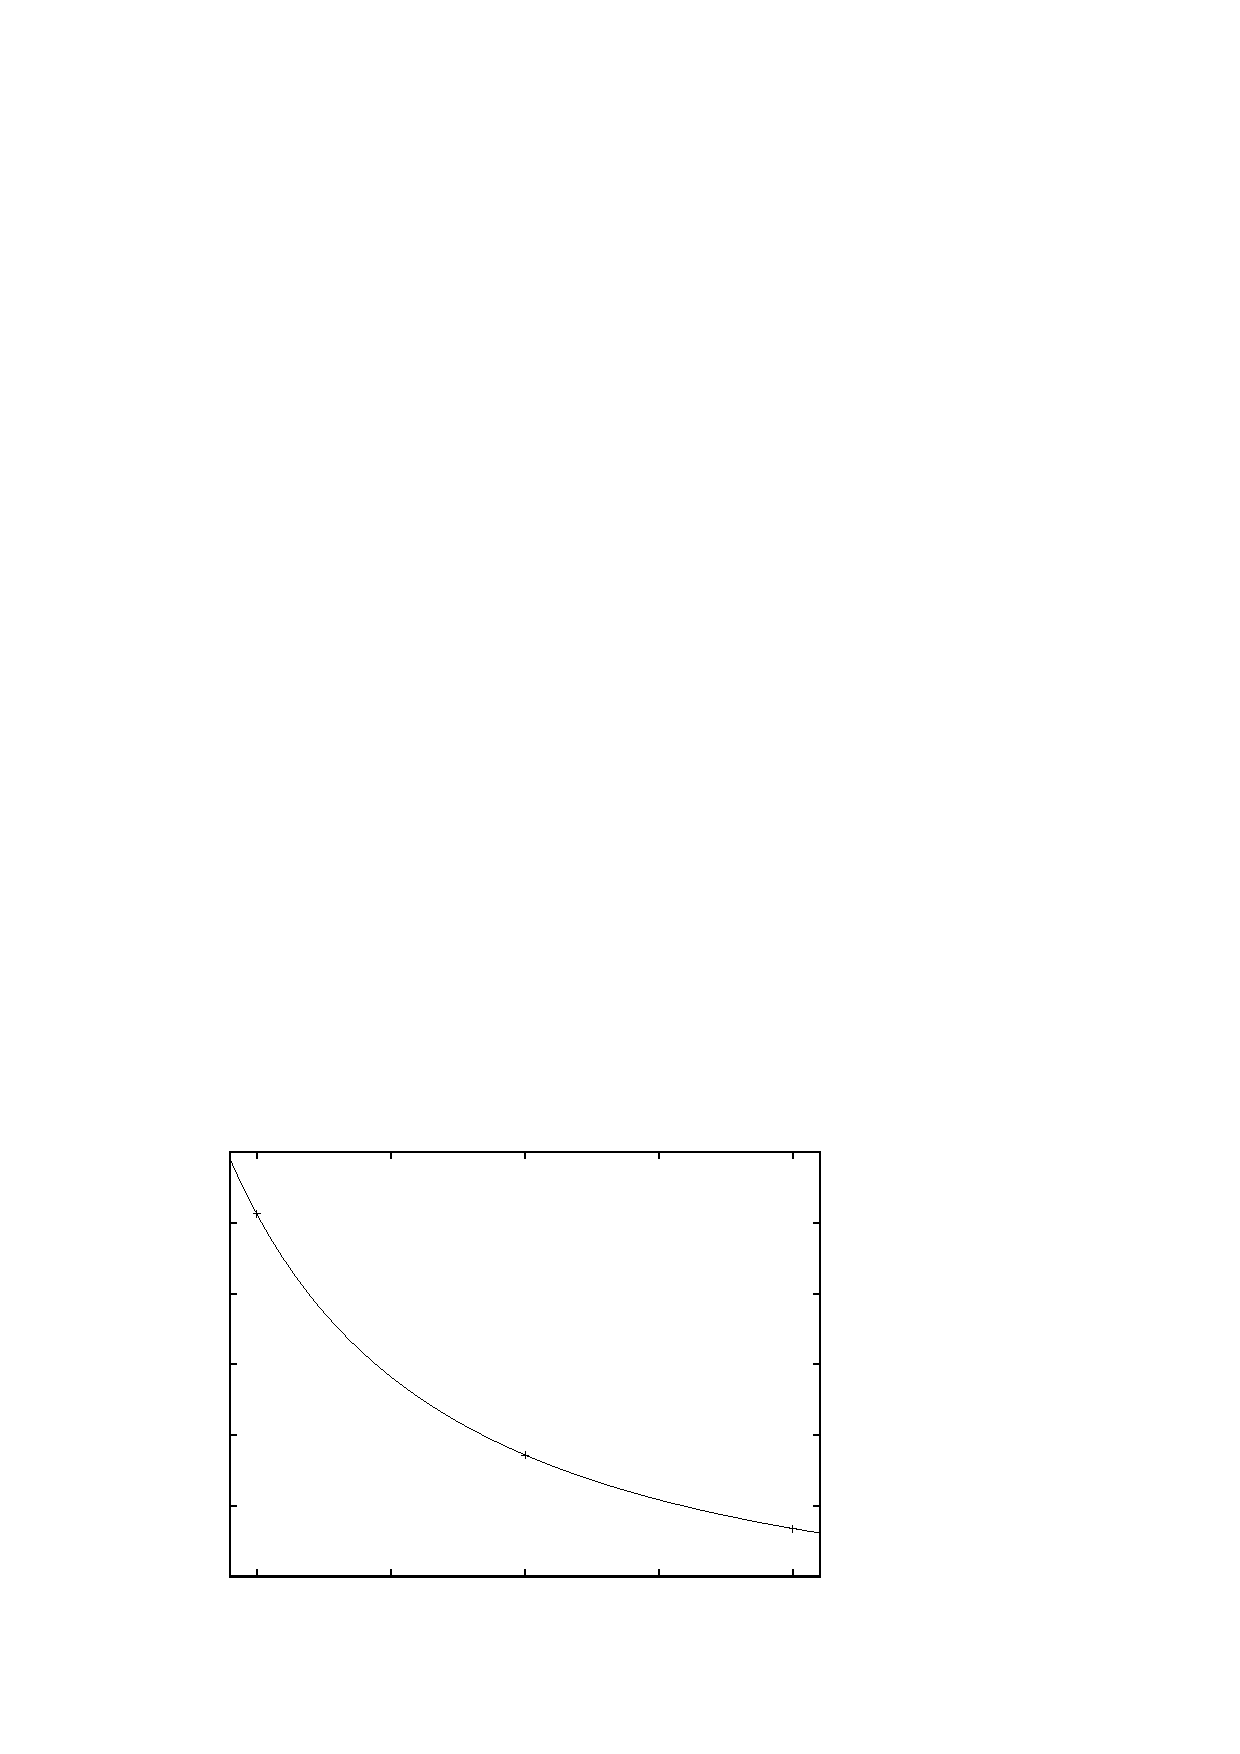
\includegraphics{GH}}%
    \gplfronttext
  \end{picture}%
\endgroup

\caption{Závislost vlnové délky čar H na $n$}
\label{GH}
\end{figure}

\section{Diskuze}
\subsection{Kalibrace}
Kalibrace byla provedena v delší oblasti, než byla dále použita pro měření, což vedlo k nižší chybě při samotném měření. Program Gnuplot sice udává chybu fitu v řádu procent až desítek procet, ale výsledná křivka dobře leží na kalibračních hodnotách.

\subsection{Rozlišoací schopnost}
Jak již bylo uvedeno výše, na spektrometru byli rozpoznatelné čáry o rozdílu až 0.04 nm. Rozlišovací schopnost může být i nižší, ale bližší čáry nebyli k dispozici. Určení rozdílu spektrálních čar se včak pohybovalo minimálně o řád níže, jak je dobře vidět na sodíkových dubletech. Na stupnici spektrometru odpovídají řádově podobným hodnotám, avšak jejich reálné rozdíly jsou značně odlišné.

\subsection{Rydbergova konstanta}
Rysbergova konstanta vyšla až překvapivě přesně. Chyba fitu byla dokonce pouhých 0.03 \%.

\section{Závěr}
Za pomoci rtuťové výbojky jsem provedl kalibraci hranolového spektrometru. Výsledná kalibrační křivka je
\begin{eqnarray}
\lambda(x)=((((3.90\cdot 10^{-15}x-2.46\cdot 10^{-11})x+ 6.73\cdot 10^{-8})x-7.49\cdot 10^{-5})x+0.0840)x+366
\end{eqnarray}
Naměřené hodnoty jsou v tabulce \ref{THg}. Kalibrační křivka je vynesena na obrázku \ref{GHg}.\\
Proměřil jsem tři dublety sodíkové výbojky a diskutoval rozlišovací schopnost spektrometru. \\
Proměřil jsem výbojky naplněné He, Ne, Ar, N$_2$ a CO$_2$. Naměřené hodnoty jsou v tabulkách \ref{THe} až \ref{TCO2}.\\
Změřil jsem vlnové délky čar vodíku z Balmerovy série a z nich určil hodnotu Rydbergovy konstanty
\begin{eqnarray}
Ry=1.0973 \cdot 10^{-7}   \mbox{m}^{-1}
\end{eqnarray} 




\begin{thebibliography}{5}
	\bibitem{text} \textbf{Studijní text na praktikum IV} \\http://physics.mff.cuni.cz/vyuka/zfp/txt\_415.pdf (13. 12. 2012)
\end{thebibliography}



\end{document}
